\newpage
\subsection{Tidal harmonic analysis of a nontidal \OGCM{}}
\label{S:plan_nontidal_tidal}

\subsubsection{Problem and motivation}
Resolving exactly what constitutes a `tidal' ocean signal is at the core of operational issues raised in the Literature Review [Section \ref{S:REVIEW}].\\
What at first appears to be a question of semantics may in fact have direct implications for the provision of sea level forecasts; especially where heterogeneous forecast systems are aggregated.\\
The premise of this study is that the sea level signal from \BL{} and conventional harmonic prediction are not mutually exclusive.  And if this is in fact the case, that aggregation should take account of this `overlap'.\\



This study aims to identify and understand what `tidal' sea level signals are present in the `nontidal' prediction system.\\
It is expected that this sub-component of the model output will include at least two distinct classes of overlap with conventional harmonic tides:
\begin{itemize}
\item periodic or quasi-periodic `meteorological' tidal constituents;
\item aperiodic `noise' (the turbulent red spectrum) that may contaminate a harmonic analysis. 
\end{itemize}


\subsubsection{Data sources}
Ultimately this study aims to understand \BL{} and inform the application of forecast aggregation.   However, it is anticipated that another directly related simulation will form the basis of this analysis - namely the multi-year \OFAM{} hindcast referred to as `the spinup run'.   In contrast to \BL{} itself, the spinup offers a longer time series produced by a constant configuration and avoids possible complications added by the effects of the data assimilation cycle.  The length of observational records are fundamental to the application of tidal analysis.\\
For comparison, observations from the ABSLMP array of coastal tide gauges [Figure \ref{fig:ABSLMP}] will be employed due to the uniquely accessible uninterrupted historical record.\\
In addition, tidal constituents produced for the Australian National Tide Tables will be referenced where relevant.

\begin{figure}[h]
\begin{center}
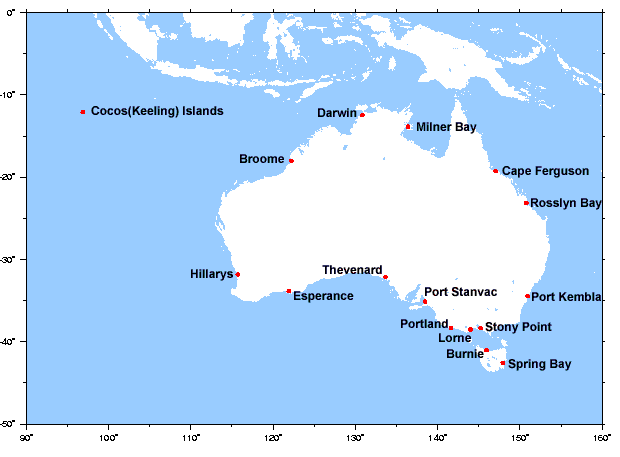
\includegraphics[width=90mm]{figures_3/map_abslmp.png}
\caption{ABSLMP sites with quality controlled data and barometric pressure observations}
\label{fig:ABSLMP}
\end{center}
\end{figure}



\subsubsection{Method outlook}
Timeseries of model output at discrete points will be compiled in the form of pseudo tide-gauge records.  At a minimum the selection of points will be aligned with the ABSLMP  array of tide gauges.  However, if computational resources allow the series of points may be extended to included a full spatial grid across the Australia region. \\

The timeseries fitting problem is formulated:\\
 $\M{A} \V{x}=\V{b}$
 where $\M{A}$ is a matrix of tidal timeseries basis functions, $\V{x}$ is the analysed tidal solution an $\V{b}$ is an observational record. \\
Use of the Singular Value Decomposition (SVD) method described by \citep{Cherniawsky:2011en} facilitates metrics addressing aspects of error and quality of fit.



It is anticipated that the available output frequency of the simulations will be a factor in preparing the data and place limitations on the analysis.   Conventional tidal practice is to analyse instantaneous hourly water level observations.   Simulation data is definitely available as daily averages, and the extent to which the more useful 3-hourly average data is available is to be determined.  Interpolation via an integral variable method is noted as a relevant tool for preparing such model output.\\
Tidal harmonic analysis will be performed on these records with a particular focus on the uncertainty bounds of any fit. It is noted that if \BL{} was in fact naively 'nontidal' then no tidal constituents would be fitted. \\



The results of these analysis will be discussed in light of the following questions: 
\begin{inparaenum}[(a)]
\item does the nominally non-tidal sea level signal project onto a tidal basis?
\item to what extent is this limited by record length and sample frequency?
\item can statistically significant tidal components be expected in \BL{}?
\end{inparaenum}



The result of this investigation will directly inform subsequent questions to be addressed in Section \ref{S:plan_insitu_analysis}\\

















